\documentclass[11pt]{article}
\usepackage[pdftex]{graphicx}
\usepackage{siunitx}
\usepackage{amsmath}
\usepackage{fixmath}
\usepackage{float}
\usepackage[czech]{babel}
\usepackage[utf8]{inputenc}
\usepackage[T1]{fontenc}
\usepackage{enumitem}
\graphicspath{ {./images/} }
\sisetup{detect-weight=true, detect-family=true}
\begin{document}

\begin{titlepage}
\center


\textbf{\Huge{Signals and systems}}
\\[4.0cm]

\textsc{\Huge {Project}}
\\[0.2cm]

\Large {Audio search system using acoustic pattern}
\\[3.0cm]

\Large{Ladislav Ondris (xondri07)}
\\[0.7cm]
\Large{19. 11. 2019}

\end{titlepage}

\newpage

\section{Recordings}
\par

\begin{center}
\begin{tabular}{ |l|l| } 
\hline
Recording & Sentence \\
\hline
sa1.wav & She had your dark suit in greasy wash water all year.  \\ 
sa2.wav & Don't ask me to carry an oily rag like that. \\ 
si1446.wav & In earlier years, the preservation of food was essentially related to survival. \\ 
si2076.wav & You gonna give me a drink, fella? \\ 
si816.wav & Do this exercise six times each class period. \\ 
sx186.wav & Would a tomboy often play outdoors? \\ 
sx276.wav & John's brother repainted the garage door. \\ 
sx366.wav & Will you please confirm government policy regarding waste removal? \\ 
sx6.wav & Bright sunshine shimmers on the ocean. \\ 
sx96.wav & Masquerade parties tax one's imagination. \\ 
\hline
\end{tabular}
\end{center}

\begin{center}
\begin{tabular}{ |c|c|c| } 
 \hline
 File name & Samples read & Length (seconds) \\ 
 \hline
 sa1.wav &  71658 & 4.478625 \\ 
 sa2.wav & 56298 & 3.518625 \\ 
 si1446.wav & 99818 & 6.238625 \\ 
 si2076.wav & 44778 & 2.798625 \\ 
 si816.wav & 65258 & 4.078625 \\ 
 sx186.wav & 52458 & 3.278625 \\ 
 sx276.wav & 60138 & 3.758625 \\ 
 sx366.wav & 78058 & 4.878625 \\ 
 sx6.wav & 51178 &  3.198625 \\ 
 sx96.wav & 60138 & 3.758625 \\ 
 \hline
\end{tabular}
\end{center}
\par 
The recordings can be used for: 
\par
c) for (a), (b) and for freely available “Czenglish TIMIT” database. 

\section{Queries}
\begin{center}
\begin{tabular}{ |c|c|c|c| } 
 \hline
 File name & Samples read & Length (seconds) & Query \\ 
 \hline
 q1.wav &  10163 & 0.635188 & essentially \\ 
 q2.wav & 10393 & 0.649563 & exercise \\ 
 \hline
\end{tabular}
\end{center}

\section{Spectogram}
\begin{figure}[H]
	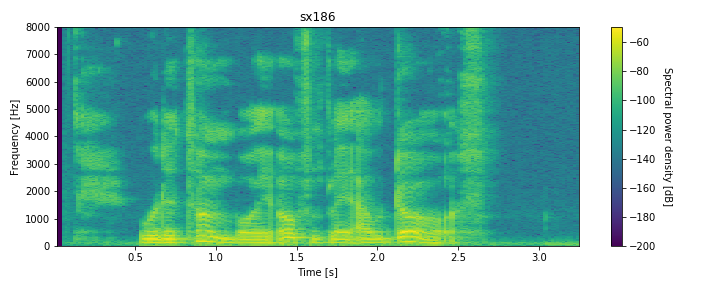
\includegraphics[width=\linewidth]{./sx186_spectogram.png}
	\caption{Would a tomboy often play outdoors?}
\end{figure}

\section{Features}
\par
I used linear bank of filters to calculate features of a given sentence or query. For that I used the matrix multiplication approach $\mathbf{F} = \mathbf{AP}$. 
\par
The purpose of matrix $\mathbf{A}$ is to sum every $B$ rows (in our case 16 rows). To make this work, we create the matrix A by filling it with zeros and ones in a specific pattern so that it produces the sum.
\par 
The first row of the matrix $\mathbf{A}$ will contain 16 ones and the rest of it will be zeros. The second row will contain 16 zeros, then 16 ones, and the rest will be zeros. And so on. 
The shape of the matrix $\mathbf{A}$ is $(B, f.size)$ where $f$ is an array of sample frequencies.

\section{Correlation score calculation}

\section{Main output}
\begin{figure}[H]
	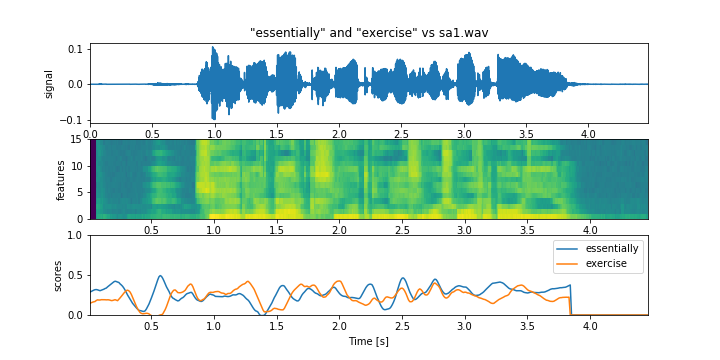
\includegraphics[width=\linewidth]{./docs/sa1.png}
\end{figure}
\begin{figure}[H]
	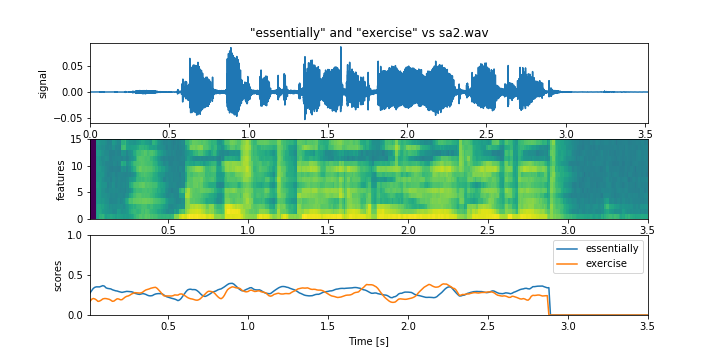
\includegraphics[width=\linewidth]{./docs/sa2.png}
\end{figure}
\begin{figure}[H]
	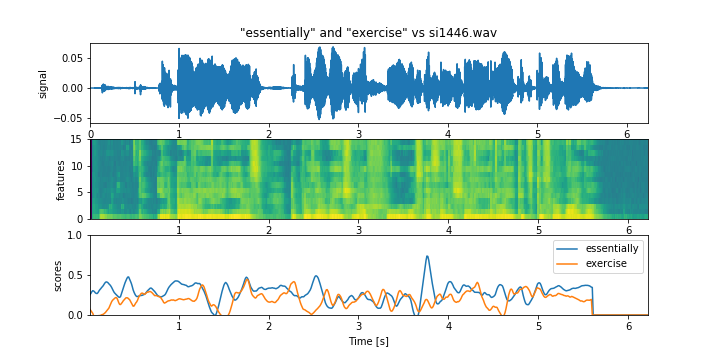
\includegraphics[width=\linewidth]{./docs/si1446.png}
\end{figure}
\begin{figure}[H]
	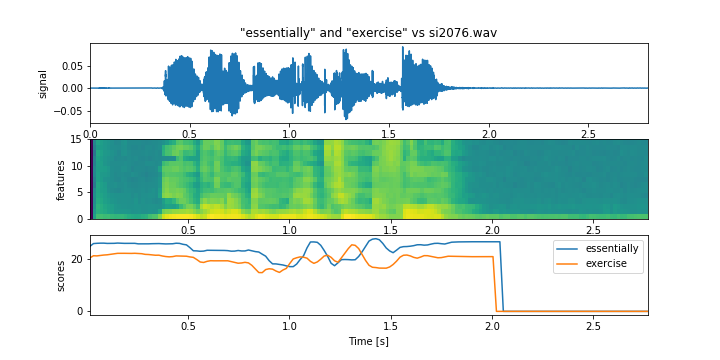
\includegraphics[width=\linewidth]{./docs/si2076.png}
\end{figure}
\begin{figure}[H]
	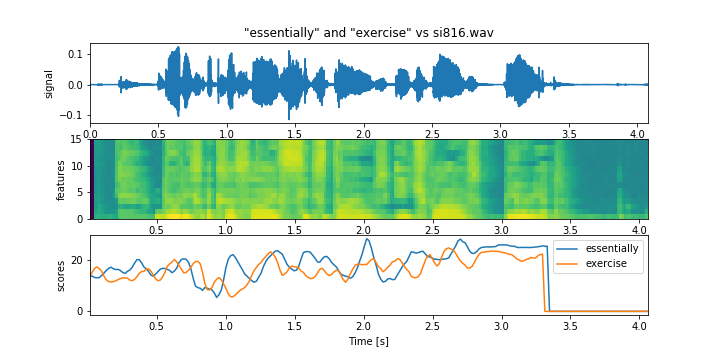
\includegraphics[width=\linewidth]{./docs/si816.png}
\end{figure}
\begin{figure}[H]
	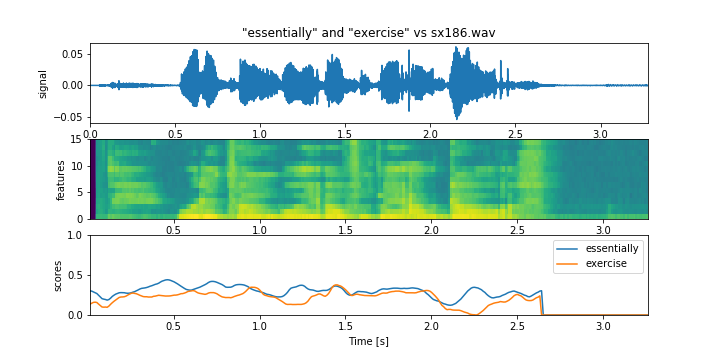
\includegraphics[width=\linewidth]{./docs/sx186.png}
\end{figure}
\begin{figure}[H]
	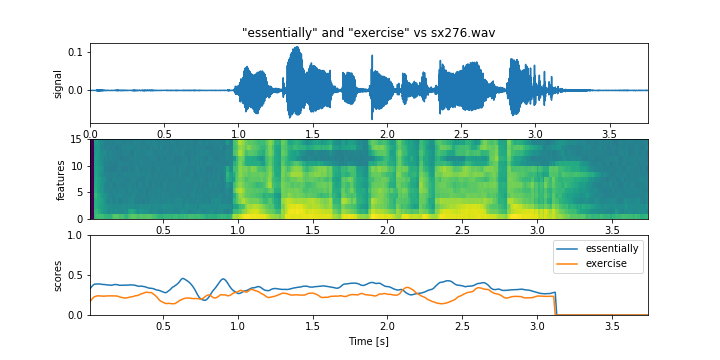
\includegraphics[width=\linewidth]{./docs/sx276.png}
\end{figure}
\begin{figure}[H]
	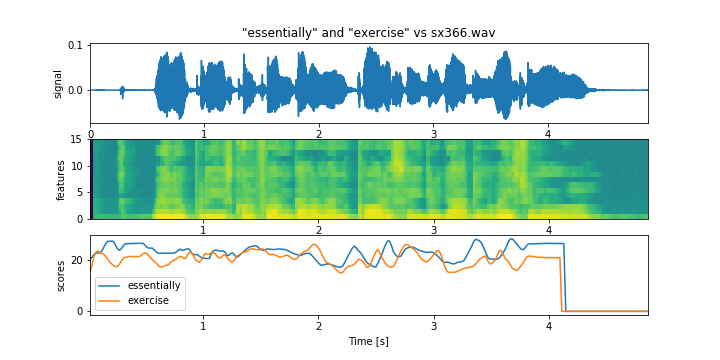
\includegraphics[width=\linewidth]{./docs/sx366.png}
\end{figure}
\begin{figure}[H]
	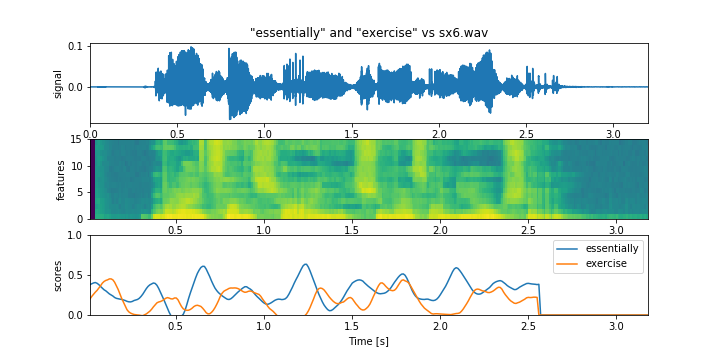
\includegraphics[width=\linewidth]{./docs/sx6.png}
\end{figure}
\begin{figure}[H]
	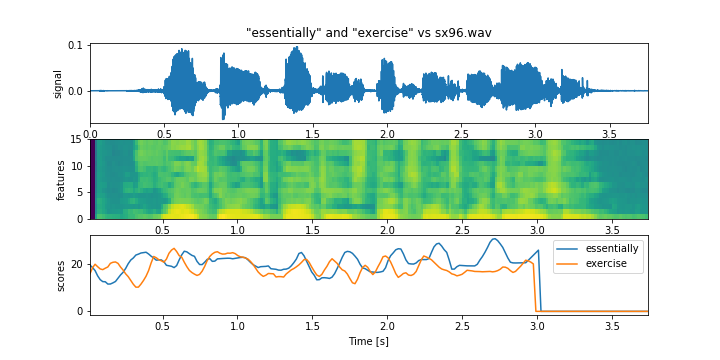
\includegraphics[width=\linewidth]{./docs/sx96.png}
\end{figure}

\section{Score evaluation}
\par
To find the occurrences of a query in the sentence, we have to specify a threshold. We can do it simply by examining the graphs of correlations for each sentense. We can easily see that it spikes in some places - these should be the occurrences of a query in a sentence.
\par
All we need to do is to find the spikes programmatically which can be done by checking whether the correlation is above the threshold and checking whether it's still ascending. Once it stops ascending, we know where the peek of the spike is and therefore the beginning of the query.

\begin{center}
\begin{tabular}{ |c|c| } 
 \hline
 Query & Threshold \\ 
 \hline
 q1.wav &  0.7 \\ 
 q2.wav & 0.6 \\ 
 \hline
\end{tabular}
\end{center}

\section{Hits}
\par
The following hits were detected using the threshold defined above. These are the correct occurrences. No incorrect were found.

\begin{center}
\begin{tabular}{ |l|c|c|c|c| }
\hline
Recording & q1.wav & q2.wav & Sample from & Sample to  \\
\hline
sa1.wav & no & no & & \\ 
sa2.wav & no & no & & \\ 
si1446.wav & yes & no & 60200 & 70160 \\ 
si2076.wav & no & no & & \\ 
si816.wav & no & yes & 13800 & 23760\\ 
sx186.wav & no & no & & \\ 
sx276.wav & no & no & &\\
sx366.wav & no & no & & \\
sx6.wav & no & no & & \\
sx96.wav & no & no & & \\
\hline
\end{tabular}
\end{center}

\section{Conclusion}
\par




\end{document}